\section{ARIFI's project description}

%The beginning of a project takes place after analysing the subject's state of the art to which it addresses. In this research, it is important to determine that the development of the project's idea will bring added value with respect to the already existing solutions. In ARIFI, we have relied on our supervisors, who are well familiarised with agriculture topics, to know from first hand some of the real difficulties farmers have, and how are they currently faced, if they are (see section X). Following up on this idea, the intention of this section is to make a more detailed comparison between ARIFI's approach to cover farmer necessities and traditional or up to date methods that are being used. We will recover the necessities presented earlier in section X and make the mentioned comparison in the following bullet-points. 
%
%
ARIFI is an ongoing project whose main goal is to combine GNSS services with Artificial intelligence into a web application. This application will provide agricultors not only with useful data, but also with instructions on what actions to take so as to manage more efficiently their farms and improve their harvest profits.\\\\
%
The project started after a several discussions with farmers from different countries around the world. Amongst all the professionals we reached, we established tighter connection with the ones presented in section \ref{adv} who up to this day constitute our advisory board. The intention of all the conversations via phone calls or e-mail, was to get a deeper insight on the state of the art concerning agriculture. We tried to analyse common difficulties among farmers, despite being far apart from one another, making special emphasis in those that we thought we could contribute to, as a team with solid knowledge in GNSS and AI.\\\\
%
%
In conclusion, we obtained valuable feedback from farmers that helped the team to better shape the project and define more clearly which difficulties we wanted to address with ARIFI. Even though out main objectives are well outlined at the moment, thanks to the potential of the technical subjects in which ARIFI is based, mainly GNSS and AI, it stands out for its scalability, which means it will be able to adapt and introduce new features relatively easily in the future.

\subsection{Interpretation of weather forecasts.}
%
It is well known that weather forecasts are of extreme importance for agriculture. It helps farmers to prevent their harvest to be damaged and also to adjust farming systems that perform vital functions such as irrigation. Farmers obtain weather forecasts, either for themselves via internet or by means of external and specialised companies. These forecastss are sometimes not precise enough. More importantly, most of them are only useful for well experienced agricultors, who knew to interpret this data and deduct what actions to take in consequence. This is a problem that ARIFI wants to solve, not only by providing more detailed weather forecasts, but also to combine them with data from other sources and time epochs to provide agricultors with instructions on how to proceed with their farming activities. We want to make from ARIFI an ally for a wide range of farmers, whatever their technical knowledge or work experience. Plus, we it can be specially useful in developing countries' agricultural sector, where consulting services from specialised companies are a limited resource.\\\\
%
%
\begin{figure}[b!]
    \centering
    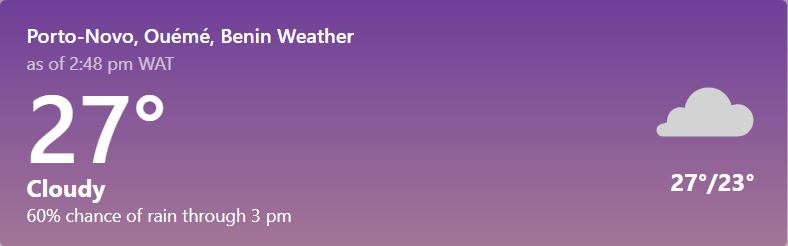
\includegraphics[scale=0.7]{images/benin.JPG}
    \caption{Porto-Novos' weather summary from weather.com}
    \label{fig:benin}
\end{figure}
%
%
Figures \ref{fig:benin}, \ref{fig:vapour}  and \ref{fig:filter} where extracted from \link{www.weather.com} and just constitute a mere example of the process a farmer should follow in order to obtain a more precise weather forecast. Figure \ref{fig:benin}, displays a climate summary from city of Porto-Novo in Benin, Africa. Figure \ref{fig:vapour} and \ref{fig:filter} display a satellite view of Porto-Novo and its surroundings with a water-vapour and an infrared filter respectively. These figures will result only useful for experienced farmers. They must know enough not only to determine the implications of the change in climate along the timeline, but also to know which actions to take in consequence, and last but not least when to take them.
%
\begin{figure}[b!]
    \centering
    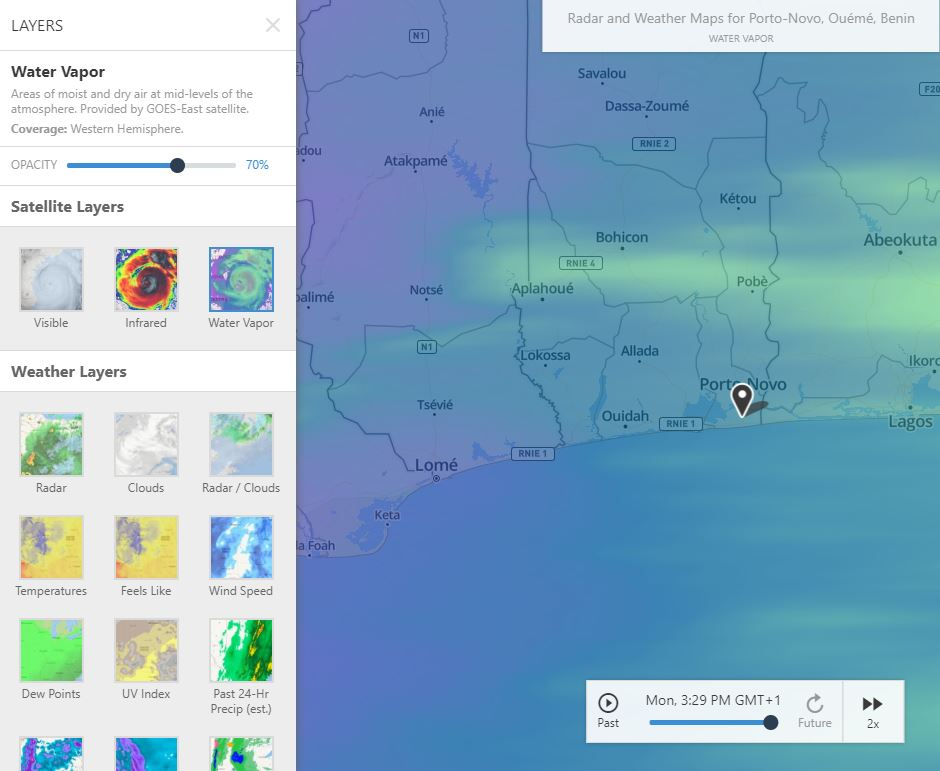
\includegraphics[scale=0.6]{images/water_vapor.JPG}
    \caption{Porto-Novos' satellite image displaying water vapour.}
    \label{fig:vapour}
\end{figure}
\begin{figure}[b!]
    \centering
    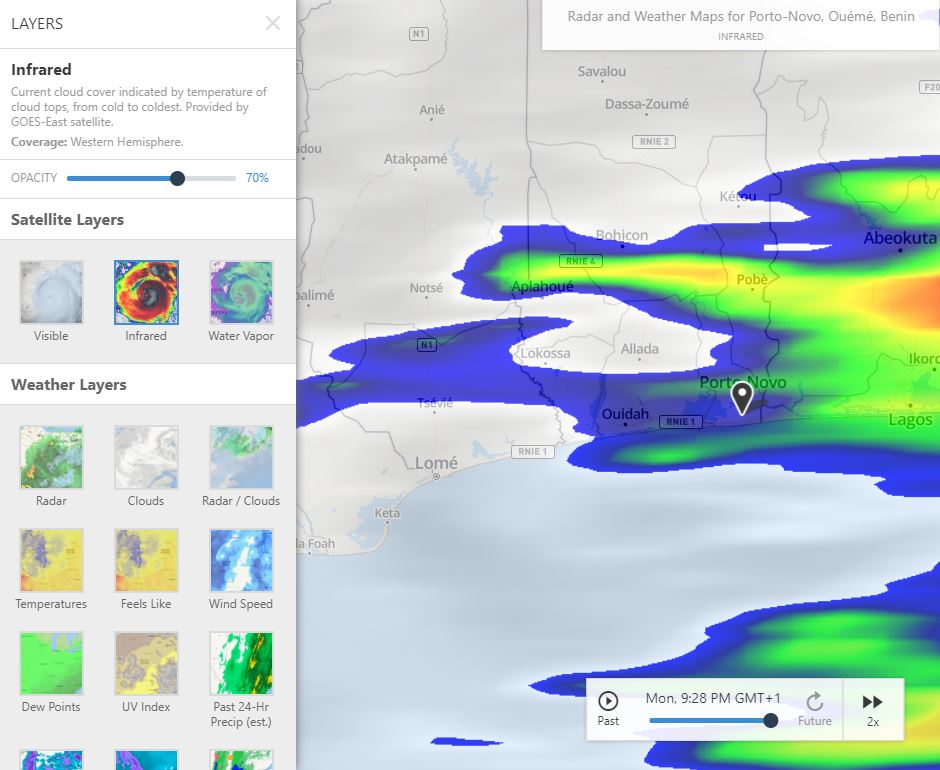
\includegraphics[scale=0.6]{images/infrared.JPG}
    \caption{Porto-Novos' satellite image with an infrared filter.}
    \label{fig:filter}
\end{figure}
\clearpage

\subsection{knowledge of field's characteristics}
Although all farmers know their fields to some extent, not many have precise and/or detailed knowledge about more concrete aspects aspects, e.g. soil height irregularities, chemical characteristics etc. These parameters should be taken into account in order to optimise many farming activities. The major handicap in this aspect is that they are not easy to determine, and in some cases it implies an expensive and time-consuming deployment of measuring devices. ARIFI expects to contribute to this necessity by offering farmers more detailed knowledge of their farms, making use of GNSS services combined with AI and signal/image processing techniques.
\subsection{Adaptation to climate change}
Climate change affects agriculture in particular by changing the intensity and duration of certain meteorologic conditions. This not only affects the way farmers have to manage their fields, but also shifts periodic climate conditions within the year, which threats agricultors' farming schedules. That being said, to optimise their harvest, farmers should not only anticipate threatening climate changes, such as heat waves, but also to adapt their yearly farming schedule to these climate shifts.
ARIFI aims to provide support to farmers in this issue by making thanks to its artificial intelligence module. The latter will keep track of climate distortions over time so as to make more accurate predictions of climate changes and shifts.  
% OVERVIEW
\subsection{Project overview}
%
\begin{figure}[b!]
    \centering
    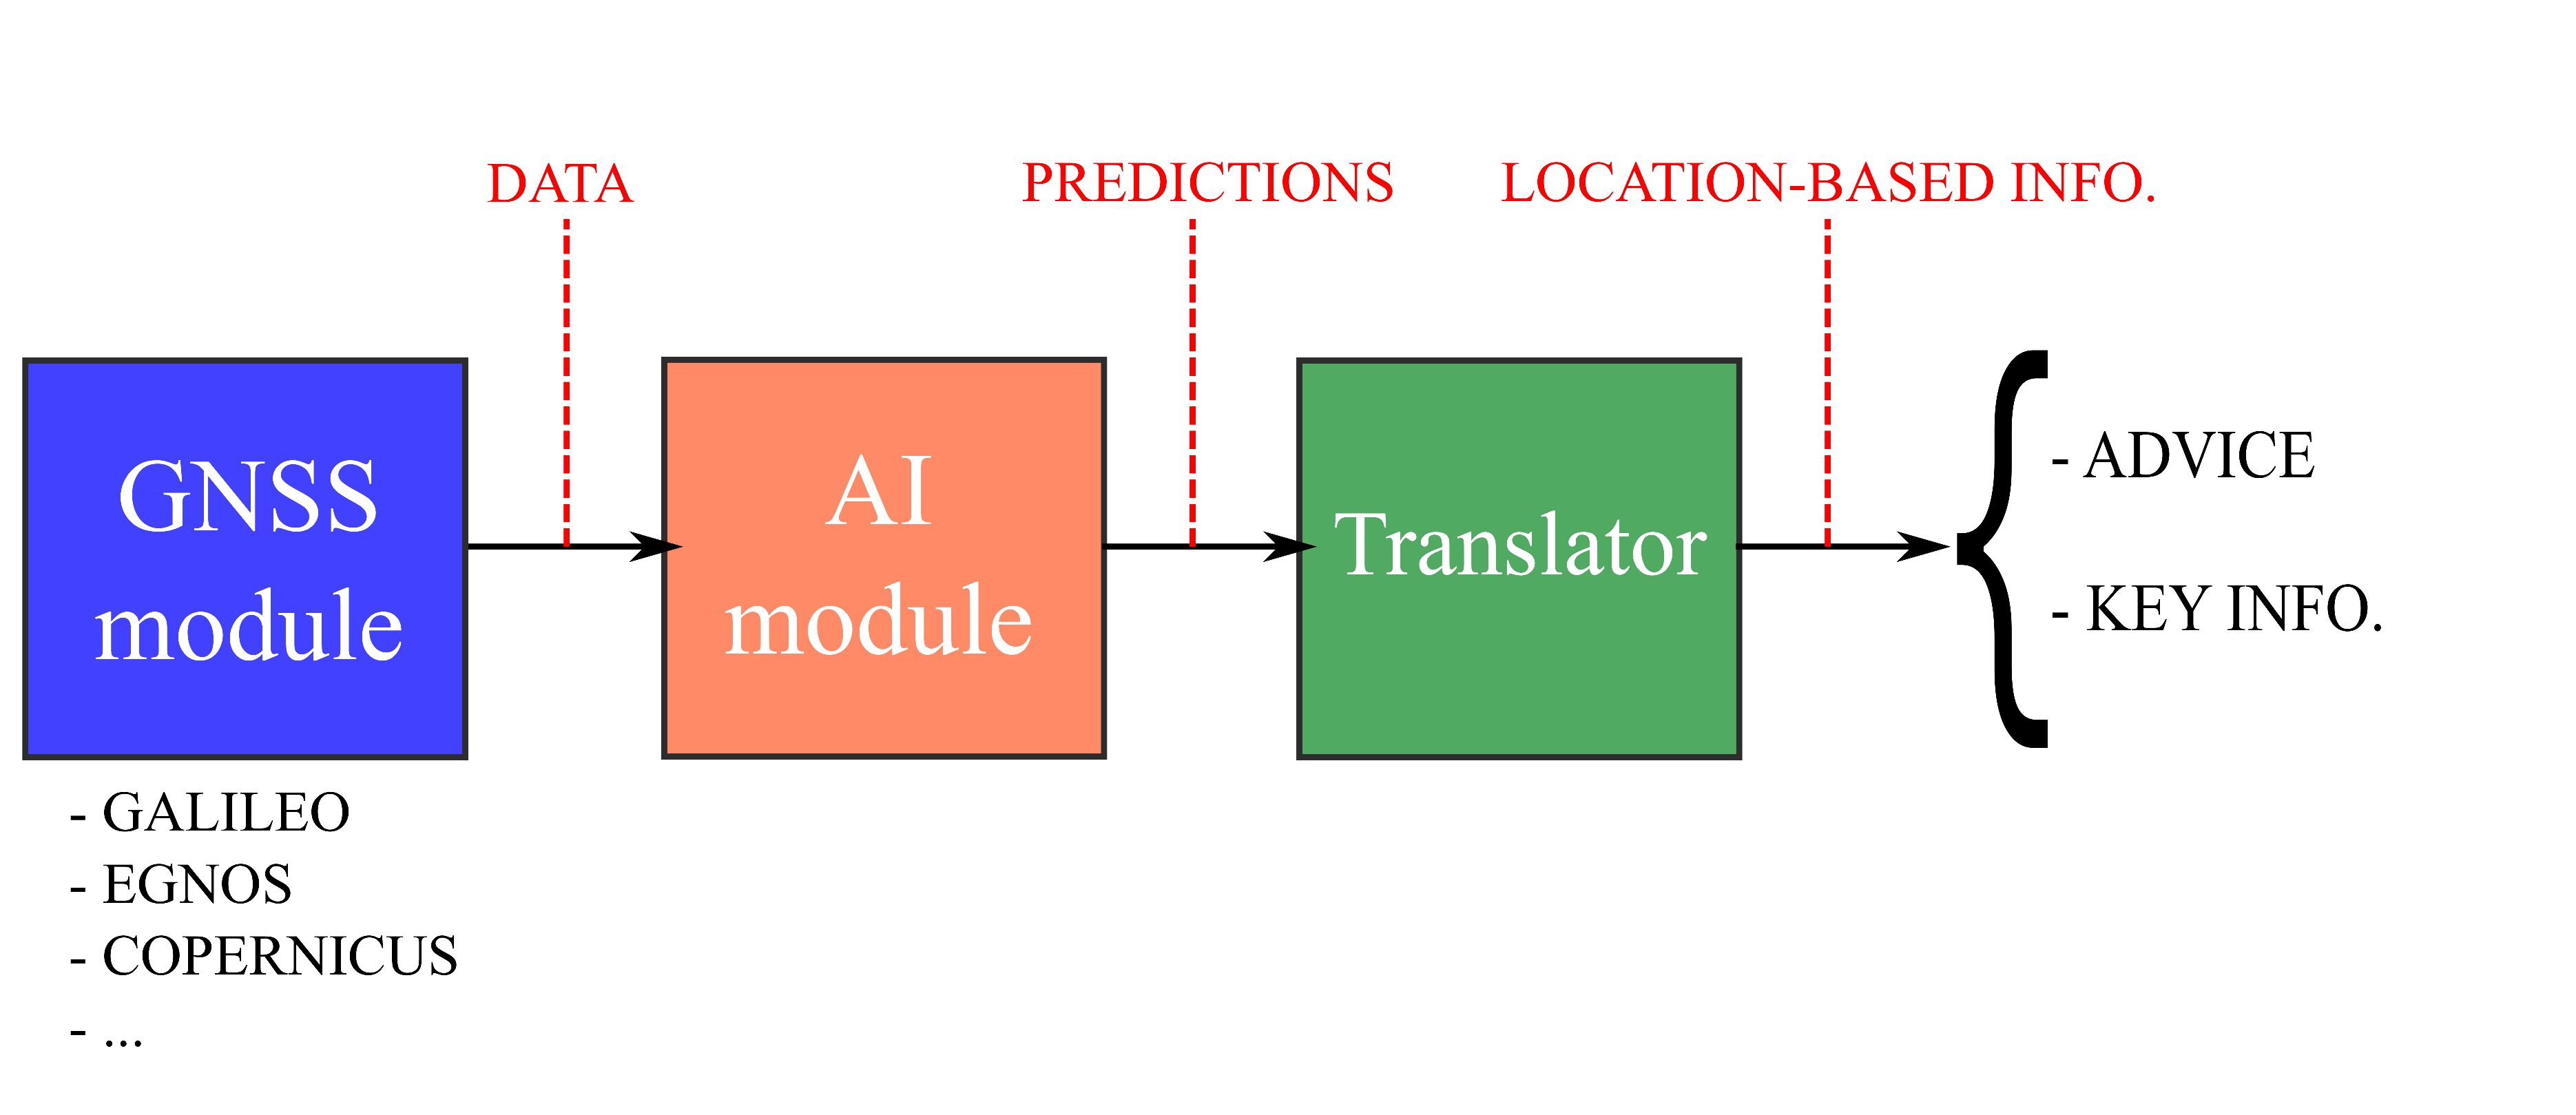
\includegraphics[scale= 0.26]{images/dibujo1.eps}
    \caption{ARIFI's general schematic}
    \label{fig:sch1}
\end{figure}
%
The principal idea is that GNSS together with other sources act as data providers to ARIFI's AI module, which will collect and integrate this information to its algorithm. Next, the AI module will output a prediction of key parameters, that will be later interpreted and made understandable for agricultors. This part is where ARIFI specially stands out from other services, as it will make special emphasis in translating AI predictions into instructions for farmers, so that their harvest follows a more efficient agricultural plan. In figure \ref{fig:sch1}, it is displayed an schematic idea of ARIFI's general concept.\\\\
%
\begin{figure}[t!]
    \centering
    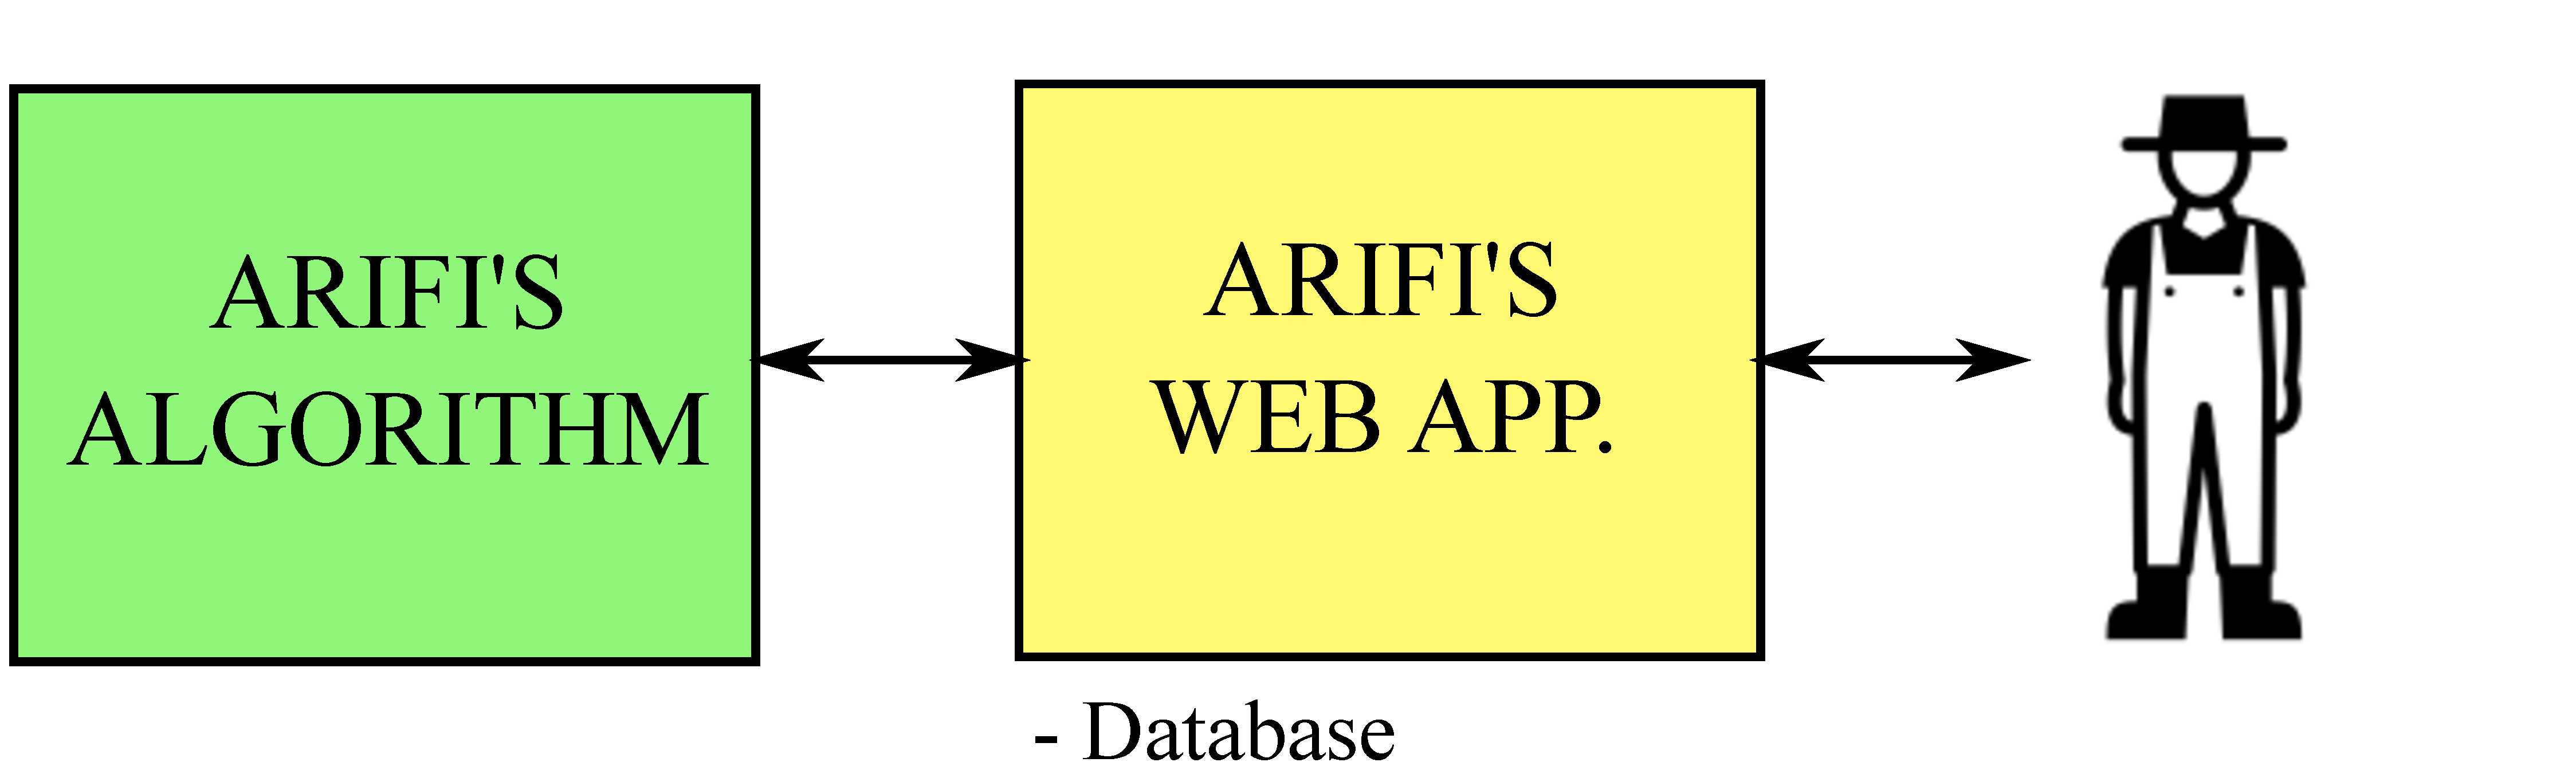
\includegraphics[scale= 0.15]{images/dibujo2.eps}
    \caption{User interaction with ARIFI's services}
    \label{fig:sch2}
\end{figure}
%
ARIFI was initially thought to work as a web application. The reason to this is that one of the major concerns from ARIFI's team, was to make this service available for a wide range of users. With this in mind, a web application was thought the best platform to work with, as it only requires a device with internet connection to access to its services. Despite this, we are opened to consider other platforms such as mobile-phone applications in the future. A graphical description of user's interaction with ARIFI is depicted in figure \ref{fig:sch2}.

\subsection{Technical aspect}
\subsubsection{Satellite services}
\begin{itemize}
    \item \textbf{GALILEO} \color{blue} is a global satellite navigation system funded, developed and maintained by Europe which provides to European citizens independence and sovereignty, minimizing the disconnection and/or interruption of other GNSS systems (such as GPS or GLONASS). Furthermore, Galileo offers new services: search and rescue (SAR), Galileo Publich Regulated Serive (PRS) for governmental authorised users and sensitive applications and more precise position for commercial purposes.   
    
    Once Galileo is fully operational it will consists of 24 active and 6 reserve satellites. Besides, different frequency bands (see figure \ref{fig:frequency_plan} \footnote{Figure obtained from \url{https://gssc.esa.int/navipedia/index.php/Galileo_Signal_Plan}}) will be used to increase and improve the precision level, availability and timing under the most hostile condition. 
    
    \begin{figure}
    	\centering
    	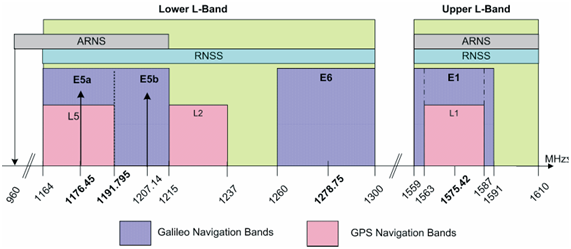
\includegraphics[width=0.8\textwidth]{images/Galileo_Frequency_Plan.png}
    	\caption{Galileo frequency distribution}
    	\label{fig:frequency_plan}
    \end{figure} 
    
    Galileo system is able to provide a position with a root-mean-square (RMS) error equals to 0.43–1.20 m, 0.52–1.29 m, and 1.34–3.25 m in the east component, north component, and up component, respectively. These errors are comparable to those obtained with GPS system despite the smaller number of satellites and larger PDOPs \cite{Gal_pos}. However, is higher accuracy is needed, a centimeter-level precision can be achieved by means of more sophisticated techniques such as precise point positioning (PPP) \cite{PPP} and  real time kinematics (RTK) \cite{RTK1, RTK2}. The former is an optimal approach for providing standalone static and kinematic geodetic point positioning solutions whereas the latter is a differential GNSS technique which provides high positioning performance in the vicinity of a base station. Although the two approaches follow a different philosophy, both make use of dual-frequency, pseudo-range and carrier-phase observable to improve the performance achieved by SPP \cite{nav_PPP, nav_RTK}.     

	Galileo, in combination with EGNOS (when this service is available), will be used by ARIFI in order to determinate the farmer's position within his farm and thus provide him with information on irregularities in the field. Therefore, a GNSS receiver which determinates the farmer's position is needed. Nonetheless, since ARIFI will has a wide world impact this receiver must be user-friendly and thinking in developing and least developed countries it should be cheap too. In this sense, in ARIFI project two alternatives are being evaluated
	\begin{itemize}
		\item A single chip GNSS mass market receiver as the developed under HIMALAYA project \cite{Himalaya}. However, a commercial solution could be too much expensive for the average farmer. 
		
		\item A software receiver developed and provided by the ARIFI team. So, the farmer would simply have to have a GNSS antenna and a platform to run the receiver. This option can be supplied at a cheaper price or even for free depending on the farmer's economical condition. 
	\end{itemize}
	  
	Regardless of the option chosen, the receiver will work under open sky conditions so it does not need to be a very sophisticated receiver since the only sources of error will be those given by the ionosphere and the troposphere (multipath can be considered negligible), and both effects can be easily corrected or at least mitigated. In the same way, given the open-sky condition more than 4 satellite can be easily acquired and tracked increasing the accuracy of the position. 
    
    
    \color{black} 

    \item \textbf{EGNOS} is satellite-based augmentation system (SBAS) of Europe and is designed to improve the performance offered by GNSS. Using three geostationary satellites, corrections and integrity information are provided to the GPS signals. The coverage that EGNOS has is practically the whole of Europe and is used for different applications and users that require this service.
    
    EGNOS provides three different services:
    
    \begin{itemize}
    
        \item Open Service (OS): the main objective is to improve the precision of the GPS signal (in the future also the GALILEO signal) through corrections related to satellite clocks, satellite position and ionospheric effects.
        
        \item Safety of Life (SoL): this service is used in critical applications such as civil aviation operations. The signal performance level in space is the most rigorous.
        
        \item EGNOS Data Acces Service (EDAS): is an access point through Internet to EGNOS data in real time and also a data history.
        
    \end{itemize}

    In this project, some of the services provided by EGNOS will be used, mainly to monitor crop and soil performance. With the EGNOS data, the spatial variability of the soil can be measured and from these data different maps of the cultivated land can be obtained. These maps will contain the necessary information to be able to accurately apply pesticides, fertilizers and water, thus obtaining a more sustainable agriculture. Another advantage that this entails is the gain of time when carrying out these tasks, achieving a more efficient agriculture.

    An example of an information map that can be offered (with the additional help of geospatial sensors on the ground) would be similar to Figure \ref{fig:egnos} where the efficiency of the terrain is represented:
    
    \begin{figure}
        \centering
        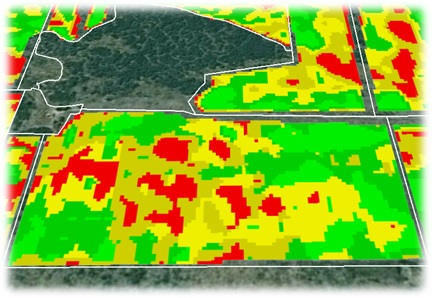
\includegraphics[width=0.8\textwidth]{images/egnos.jpg}
        \caption{Terrain efficiency map}
        \label{fig:egnos}
    \end{figure} 
    
    It has been studied that the use of these services in agriculture have a series of advantages and that is why it has been considered to use EGNOS for this project. One of the things that makes this service attractive is that it is completely free and does not require additional hardware installation on farms or agricultural work fields. It is also very interesting since the information received is information in real time thanks to the three geostationary satellites. Finally, EGNOS is widely available, allowing the farmer to be able to use the service at all times.
    
    \item \textbf{Copernicus} is a space program promoted by ESA and its main objective is to provide land surface data to improve environmental management and mitigate the effects of climate change, among other applications.
    
    Copernicus is composed of a network of sensors positioned around the Earth and 6 different groups of satellites (the Sentiel) that provide terrestrial observations and measurements, such as images of weather conditions, high-resolution multispectral optical images, atmospheric composition, air quality, etc.
    
    It has been considered to make use of the data provided by Copernicus, specifically from the second group of satellites (Sentinel 2) which provide multispectral optical images, very useful in the field of agriculture. These satellites pass every 5 days, therefore the farmer will be able to have information about his crop every this period of time with a resolution of 10x10m. An example of the images that these satellites provide can be seen in Figure \ref{fig:copernicus}.
    
    \begin{figure}
        \centering
        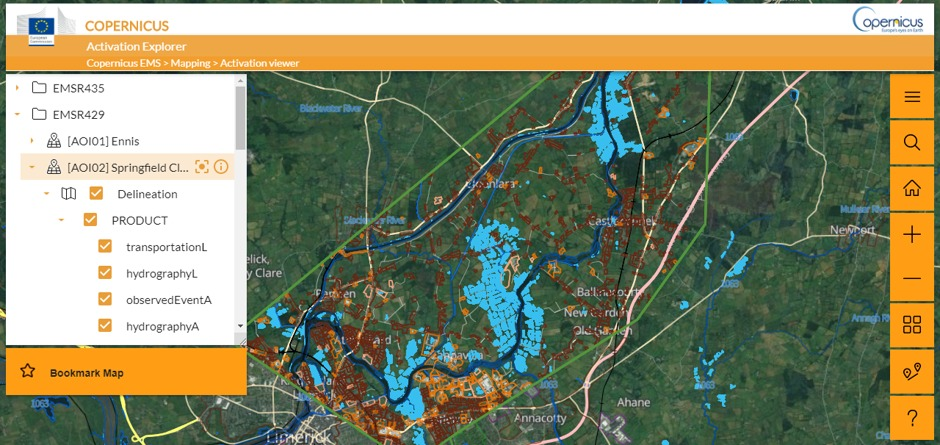
\includegraphics[width=0.8\textwidth]{images/copernicus.jpeg}
        \caption{Image provided by Copernicus}
        \label{fig:copernicus}
    \end{figure} 
    
    A variable that will be extracted from this service is the Normalized Difference Vegetation Index (NDVI) that is used to estimate the quantity, quality and development of vegetation based on the measurement of radiation intensity of certain bands of the electromagnetic spectrum. that the vegetation emits or reflects. With this parameter the area can be mapped highlighting the parts of the land that need to be fertilized, areas affected by diseases or pests and areas with water deficits.
    
    Therefore, the use of the service provided by this program will serve to optimize resources, predict crop performance and save time when inspecting the crop and acting on problems on soil problems.
    
\end{itemize}
\subsubsection{Artificial intelligence}
To address the proposed idea and achieve our goal, we will focus on how to relate machine learning techniques, field of Artificial Intelligence (AI), with the study of the atmosphere provided by satellite data. Thanks to the Copernicus Atmosphere Monitoring Service, we will be able to access to data that will allow us to predict the main atmospheric phenomenons which affects the production of the majority farmers.\\\\
%
In particular, we are talking about reanalysis variables. This kind of data is obtained by some weather forecasting centres, which combine past observations with a modern meteorological forecast model, in order to produce regular gridded datasets of many atmospheric and oceanic variables, with a temporal resolution of a few hours. This datasets usually extend over several decades and cover the entire planet, being a very useful tool for meteorological and climatological studies.\\\\
%
One of the most important reanalysis projects is the {\em ERA-Interim reanalysis project}, produced by the European Centre for Medium-Range Weather Forecasts (ECMWF) \cite{ERA_Interim}, which belongs to the Copernicus Programme. ERA-Interim is a global atmospheric reanalysis from 1979, continuously updated in real time.\\\\
%
Table \ref{Variables_ERA} is just an example of variables that can be obtained from this platform, which could be used as predictors in machine learning models.

\vspace{12pt}
\begin{table}[H]
\begin{center}
\caption{\label{Variables_ERA} Possible predictive variables in a prediction problem.}
\begin{tabular}{cccc}
\hline
variable name & ERA-Interim variable\\
\hline
\hline
skt & surface temperature\\
sp & surface pression\\
$u_{10}$& zonal wind component ($u$) at 10m\\
$v_{10}$& meridional wind component ($v$) at 10m\\
temp1& Temperature at 500hPa\\
up1& zonal wind component ($u$) at 500hPa\\
\hline
\end{tabular}
\end{center}
\end{table}
\vspace{12pt}

Due to the chaotic nature of atmospheric phenomenons it is so difficult predict with precision its future state. Modeling it without any un- certainty is not possible as there is a strong sensitivity to small perturbations in the initial conditions. But there is a way to overcome this issue by the use of probabilistic weather forecasts \cite{martinez2015forecasting}. In this regard, we propose computational methods belonging to machine learning techniques, a branch of AI, to get predictions or classifications over the main atmospheric factors with high accuracy. We could predict solar radiation, wind velocity, or whatever meteorological process that injures in the farmers' environment. Of course, it would not be possible without GNSS services that provide the essential dataset, as we mentioned before, necessary to train the learning models.

Many of these methods can be classified in the field of Knowledge called “Natural Computing”. The algorithms that can be found in this category are inspired by the way Nature solves complex problems. In this regard, Evolutionary Computation (EC) is inspired in the theory of evolution or Artificial Neural Networks (ANN) find their behaviour in human brain.

The conjunction between satellite data and machine learning algorithms will allow us to provide solutions to those aspects that most concern farmers, in order to keep their harvests safe with the highest possible productivity. For instance, if we are able to anticipate how much water they will have at a given time, or to warn of a dry season that was not previously contemplated but, due to the effects produced by climate change may occur, we will have a positive influence on their economy by avoiding unnecessary expenses derived from poor management, because they do not have all the information they could.

\subsection{Schedule}
ARIFI's project plan follows the GSA Farming by satellite schedule. The latter consists of the 3 phases listed bellow, which have been also displayed in figure X for a more graphical description.
\begin{figure}[b!]
\centering
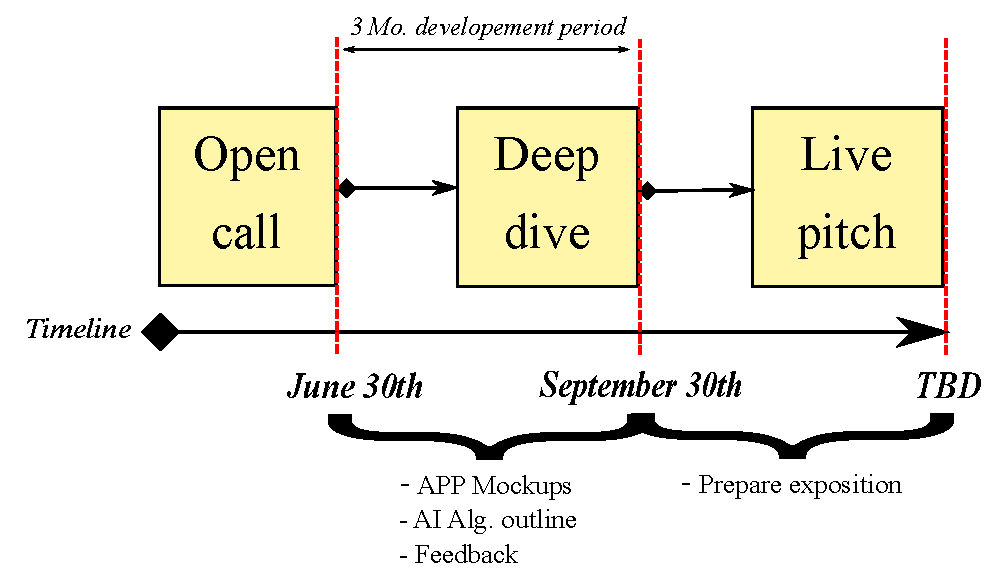
\includegraphics[scale= 0.7]{images/schedule.eps}
\caption{ARIFI's timeline within the GSA contest}
\label{fig:sch2}
\end{figure}
\begin{enumerate}
    \item \textbf{Open call for ideas:} In this phase we worked hard so as to give shape to our project idea. To do this, we kept close contact with our advisory board with a high degree of expertise in agriculture. 
    \item \textbf{Deep Dive Phase:} In this phase we expect to outline more concrete details about ARIFI, also taking advantage from GSA advice. The list of pending subjects we have left for the deep dive phase are the following:
    \begin{itemize}
        \item \textbf{Web Application Interface:} We expect to define a primary web interface so that reviewers can have a feeling of how will the user interaction with the app be. We expect to make an accurate mock-up similar to the final version.
        \item \textbf{AI algorithm:} Our expert in AI has described how should the AI algorithm work so as to output key data, that will later be required from consecutive modules. However, more work is needed in this subject so as to define and adapt more accurately this concrete module to project as a whole.
        \item \textbf{Advisor's supervision:} We do not forget that in order to achieve ARIFI's success, we should keep in constant contact with our advisors and take experts feedback into account, so as to avoid drifting off the initial objective and cover farmer necessities.
    \end{itemize}
    \item \textbf{Live Pitches:} After presenting our work from the deep dive face, we will count with a yet to be determined period of time to create our live pitch exposition and to prepare ARIFI's presentation.\\
\end{enumerate}



